\documentclass[conference]{IEEEtran}
\IEEEoverridecommandlockouts
% The preceding line is only needed to identify funding in the first footnote. If that is unneeded, please comment it out.
\usepackage{cite}
\usepackage{amsmath,amssymb,amsfonts}
\usepackage{algorithmic}
\usepackage{graphicx}
\usepackage{textcomp}
\usepackage{xcolor}
\def\BibTeX{{\rm B\kern-.05em{\sc i\kern-.025em b}\kern-.08em
    T\kern-.1667em\lower.7ex\hbox{E}\kern-.125emX}}
\begin{document}

\title{End Semester Assignment\\
{\footnotesize 17/06/2021}
}

\author{\IEEEauthorblockN{ Chella Thiyagarajan N}
\IEEEauthorblockA{\textit{ME17B179} \\
\textit{me17b179@smail.iitm.ac.in}}
}

\maketitle

\section{Question 1}
\subsection{Part (a)}
Mass-Damper system having atleast 5 nodes:
\begin{figure}[htbp]
\centerline{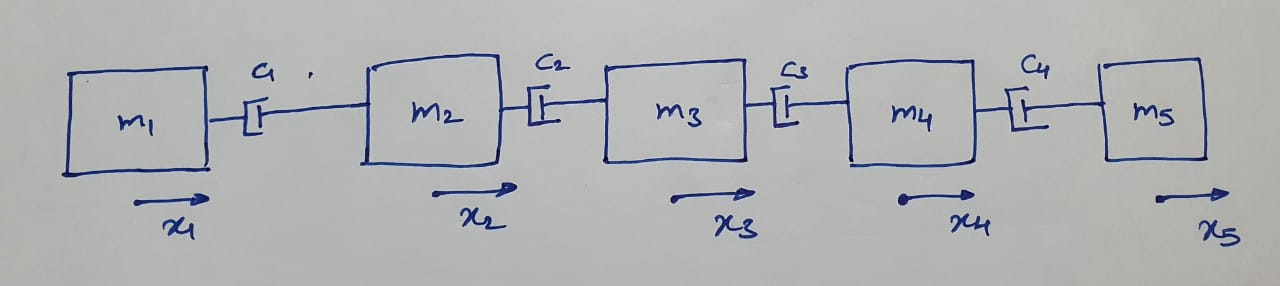
\includegraphics[scale=0.2]{img11.jpeg}}
\caption{Mass Damper system with 5 nodes}
\label{fig4}
\end{figure}

Assumed damping coefficients are = 
\[
\begin{bmatrix}
    c_1\\
    c_2\\
    c_3\\
    c_4\\
    c_5\\
\end{bmatrix}
=
\begin{bmatrix}
    10\\
    20\\
    30\\
    40\\
    50\\
\end{bmatrix}
\]
\newline

The System equations corresponding to the above system:
\begin{enumerate}
    \item $ m_1\ddot x_1 + c_1(\dot x_1-\dot x_2) = 0 $
    \item $ m_2\ddot x_2 + c_1(\dot x_2-\dot x_1) + c_2(\dot x_2-\dot x_3) = 0 $
    \item $ m_3\ddot x_3 + c_2(\dot x_3-\dot x_2) + c_3(\dot x_3-\dot x_4) = 0 $
    \item $ m_4\ddot x_4 + c_3(\dot x_4-\dot x_3) + c_4(\dot x_4-\dot x_5) = 0 $
    \item $ m_5\ddot x_5 + c_4(\dot x_5-\dot x_4) = 0 $
\end{enumerate}

System Equations Matrix Form:
\[
\begin{bmatrix}
    m_1\ddot x_1\\
    m_2\ddot x_2\\
    m_3\ddot x_3\\
    m_4\ddot x_4\\
    m_5\ddot x_5\\
\end{bmatrix}
\]
\[
=
\begin{bmatrix}
    -c_1 & c_1 & 0 & 0 & 0\\
    c_1 & -(c_1+c_2) & c_2 & 0 & 0\\
    0 & c_2 & -(c_2+c_3) & c_3 & 0\\
    0 & 0 & c_3 & -(c_3+c_4) & c_4\\
    0 & 0 & 0 & c_4 & -c_4\\
\end{bmatrix}
\begin{bmatrix}
    \dot x_1\\
    \dot x_2\\
    \dot x_3\\
    \dot x_4\\
    \dot x_5\\
\end{bmatrix}
\]
\subsection{Part (b)}
The matrix form from the previous subsection resembles the equation given in example 3.1
\[\dot p = -DR{D^T}{M^{-1}}p\]
where 
\[\dot p = 
\begin{bmatrix}
    m_1\ddot x_1\\
    m_2\ddot x_2\\
    m_3\ddot x_3\\
    m_4\ddot x_4\\
    m_5\ddot x_5\\
\end{bmatrix}
\]
\[M^{-1}p = 
\begin{bmatrix}
    \dot x_1\\
    \dot x_2\\
    \dot x_3\\
    \dot x_4\\
    \dot x_5\\
\end{bmatrix}
\]
\[ -DR{D^T} = 
\begin{bmatrix}
    -c_1 & c_1 & 0 & 0 & 0\\
    c_1 & -(c_1+c_2) & c_2 & 0 & 0\\
    0 & c_2 & -(c_2+c_3) & c_3 & 0\\
    0 & 0 & c_3 & -(c_3+c_4) & c_4\\
    0 & 0 & 0 & c_4 & -c_4\\
\end{bmatrix}
\]

with p the vector of momenta of the masses associated to the
vertices, M the diagonal mass matrix, R the diagonal matrix of
damping coefficients of the dampers attached to the edges, and
$H(p) = ({p^T}{M^{-1}}p)/2$ the total kinetic energy of the masses. The
vector of velocities $v = {M^{-1}}p$ converges to a vector in the kernel
of L = $DR{D^T}$.
By substituting damper coefficient values in $DR{D^T}$ matrix we get:
\[L = 
\begin{bmatrix}
    10 & -10 & 0 & 0 & 0\\
    -10 & 30 & -20 & 0 & 0\\
    0 & -20 & 50 & -30 & 0\\
    0 & 0 & -30 & 70 & -40\\
    0 & 0 & 0 & -40 & 40\\
\end{bmatrix}
\]

\subsection{Part (c)}
Proposition 4.2: The flow-Laplacian matrix L satisfies $L + {L^T} >= 0$ if and only if it is balanced; that is, not only ${\mathbf{1}^T}L = 0$ (column sums zero) but also $L{\mathbf{1}} = 0$ (row sums zero).
\newline
I have implemented $L + {L^T} >= 0$, ${\mathbf{}{1}^T}L = 0$ and $L{\mathbf{}{1}} = 0$ in python code and all the conditions are satisfied.
Therefore L is balanced.
\newline
\newline
Note: Please refer to Question\_1.ipynb jupyter notebook for code and further details

\section{Question 2}
I have used isl\_wise\_train\_detail\_03082015\_v1.csv file outsourced by Indian Railways. I have constructed a directed graph with station nodes which are immediately connected by a train without any intermediate stations, while the weights on edges represent the number of trains directly linking two stations. My constructed graph has 4344 station nodes and 16992 directed edges.

\subsection{Part (a)}
Average path length is a concept in network topology that is defined as the average number of steps along the shortest paths for all possible pairs of network nodes. It is a measure of the efficiency of information or mass transport on a network.Average path length is one of the three most robust measures of network topology, along with its clustering coefficient and its degree distribution. The average path length distinguishes an easily negotiable network from one, which is complicated and inefficient, with a shorter average path length being more desirable. However, the average path length is simply what the path length will most likely be. The network itself might have some very remotely connected nodes and many nodes, which are neighbors of each other.
Average path length is calculated for weekly connected components. As a fact our network has 3 weekly connected components.
Results = 
\begin{enumerate}
\item Weakly Connected Component 1
\begin{enumerate}
\item Number of Nodes = 4328
\item Number of Directed Edges = 16967
\item Average Path Length = 7.85583
\end{enumerate}
\item Weakly Connected Component 2
\begin{enumerate}
\item Number of Nodes = 8
\item Number of Directed Edges = 11
\item Average Path Length = 1.57142
\end{enumerate}
\item Weakly Connected Component 3
\begin{enumerate}
\item Number of Nodes = 8
\item Number of Directed Edges = 14
\item Average Path Length = 3.0
\end{enumerate}
\end{enumerate}
The max value of average path length is around 8 which gives us the insight that in India any station can be reached from any station in 8 steps or trains. Which really shows that how interconnected our whole railway network is inorder to connect major cities and rurals from Jammu to Kanyakumari.

\subsection{Part (b)}
It is the shortest distance between the two most distant nodes in the network. In other words, once the shortest path length from every node to all other nodes is calculated, the diameter is the longest of all the calculated path lengths. The diameter is representative of the linear size of a network.
Network Diameter is calculated for Strongly connected components. As a fact our network has 13 weekly connected components.
Results = 
\begin{enumerate}
\item Strongly Connected Component 1
\begin{enumerate}
\item Number of Nodes = 1
\item Number of Directed Edges = 0
\item Network Diameter = 0
\end{enumerate}
\item Strongly Connected Component 2
\begin{enumerate}
\item Number of Nodes = 1
\item Number of Directed Edges = 0
\item Network Diameter = 0
\end{enumerate}
\item Strongly Connected Component 3
\begin{enumerate}
\item Number of Nodes = 1
\item Number of Directed Edges = 0
\item Network Diameter = 0
\end{enumerate}
\item Strongly Connected Component 4
\begin{enumerate}
\item Number of Nodes = 1
\item Number of Directed Edges = 0
\item Network Diameter = 0
\end{enumerate}
\item Strongly Connected Component 5
\begin{enumerate}
\item Number of Nodes = 1
\item Number of Directed Edges = 0
\item Network Diameter = 0
\end{enumerate}
\item Strongly Connected Component 6
\begin{enumerate}
\item Number of Nodes = 4321
\item Number of Directed Edges = 16960
\item Network Diameter = 35
\end{enumerate}
\item Strongly Connected Component 7
\begin{enumerate}
\item Number of Nodes = 1
\item Number of Directed Edges = 0
\item Network Diameter = 0
\end{enumerate}
\item Strongly Connected Component 8
\begin{enumerate}
\item Number of Nodes = 1
\item Number of Directed Edges = 0
\item Network Diameter = 0
\end{enumerate}
\item Strongly Connected Component 9
\begin{enumerate}
\item Number of Nodes = 1
\item Number of Directed Edges = 0
\item Network Diameter = 0
\end{enumerate}
\item Strongly Connected Component 10
\begin{enumerate}
\item Number of Nodes = 1
\item Number of Directed Edges = 0
\item Network Diameter = 0
\end{enumerate}
\item Strongly Connected Component 11
\begin{enumerate}
\item Number of Nodes = 1
\item Number of Directed Edges = 0
\item Network Diameter = 0
\end{enumerate}
\item Strongly Connected Component 12
\begin{enumerate}
\item Number of Nodes = 5
\item Number of Directed Edges = 8
\item Network Diameter = 4
\end{enumerate}
\item Strongly Connected Component 1
\begin{enumerate}
\item Number of Nodes = 8
\item Number of Directed Edges = 14
\item Network Diameter = 7
\end{enumerate}
\end{enumerate}
Maximum diameter in our Indian Railway network is 35 which is a very big number of steps to reach most apart stations in our network, this tells about the corner cases that our Railway network lacks and sheds some light on future developments.

\subsection{Part (c)}
I have found 3 weakly connected components and 13 strongly connected components from our Indian Railways network. More than one weakly connected components tells us that there are stations which are impossible to reach or travel from, but from our previous analysis majority of the station are under one big network, only 2 disjoint 8 station networks are the other two, so this doesn't cause big disadvantages to the inter connectivity all over India. But the problem is that we have more than 3 strongly connected components which needs to be looked into.

\subsection{Part (d)}
I have considered four centrality measures among all the centrality measures available. These centrality's were chosen with our coursework and previous assignments in mind. Chosen Centrality's are

\begin{enumerate}
\item Degree Centrality
\item Eigen Vector Centrality
\item Katz Centrality
\item Pagerank Centrality
\end{enumerate}
katz centrality uses $\alpha$ = 1/(2*$\rho$) where $\rho$ is the maximum value of the spectrum of adjacency matrix. Pagerank centrality uses $\alpha$ = 0.5.
I have calculated all the above mentioned 4 centralities for every node available in the Indian Railways network and stored them as excel sheets as follows 
\begin{enumerate}
\item q2\_degree\_centrality.xlsx
\item q2\_eigen\_vector\_centrality.xlsx
\item q2\_katz\_centrality.xlsx
\item q2\_pagerank\_centrality.xlsx
\end{enumerate}

\newline
\newline
Note: Please refer to Question\_2.ipynb jupyter notebook for code and further details

\section{Question 3}
I have considered 57buses dataset for this problem. Important part of this question is to calculate average controllability centrality using the given paper. Given a complex network with n nodes and an associated stable linear dynamics matrix A, the Average Energy Controllability Centrality measure for node i is given by
\[ C_{CE}(i) = tr(W_i)\]
where \[W_i\] is the infinite-horizon controllability Gramian that satisfies \[AW_i + W_i A^T + e_i (e_i)^T = 0\]
where $e_i$ has a 1 in the $i^{th}$ entry and zeros elsewhere. The tricky part here is to calculate the stable system matrix A. I have explored other related papers that could shed more light on calculating system matrix A. Grid stabilization through VSC-HVDC using wide area measurements by Alexander Fuchs provides more knowledge about the relation ship between Y and A matrix and the method to calculate Y matrix. However TA has facilitated us by providing the Y matrix through prebuilt matlab functions.
I have taken the given Y matrix and calculated laplacian matrix of Y to achieve the system matrix A. Later this matrix is used to calculate $W_i$ for each i or bus in the European Grid network. trace of each $W_i$ provides us the Average Energy Controllability Centrality measure for each bus. Finally I have chosen 10 best locations that maximize average controllability, as discussed in the paper. Those 10 best locations are
\begin{enumerate}
\item 31
\item 33
\item 32
\item 30
\item 19
\item 20
\item 57
\item 42
\item 25
\item 56
\end{enumerate}


Note: Please refer to Question\_3.ipynb jupyter notebook for code and further details

\section{Question 4}
Directed graph has been constructed for the given edge connections and given weights. The graphical visualization of the given DiGraph:

\begin{figure}[htbp]
\centerline{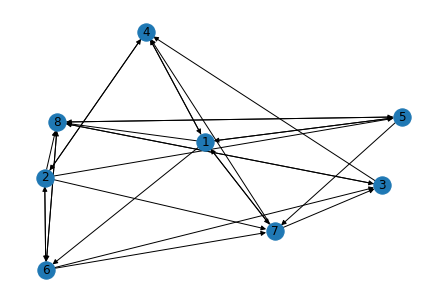
\includegraphics[scale=0.6]{img41.png}}
\caption{Given DiGraph}
\label{fig1}
\end{figure}

It's respective adjacency matrix:
\[
A = 0.015(
\begin{bmatrix}
    0 & 1 & 1 & 1 & 1 & 1 & 0 & 0\\
    1 & 0 & 0 & 0 & 0 & 0 & 1 & 0\\
    1 & 0 & 0 & 0 & 1 & 1 & 0 & 0\\
    0 & 0 & 0 & 0 & 1 & 1 & 1 & 1\\
    1 & 1 & 0 & 0 & 0 & 0 & 0 & 1\\
    0 & 0 & 1 & 1 & 0 & 0 & 0 & 1\\
    0 & 1 & 1 & 1 & 1 & 1 & 0 & 0\\
    0 & 1 & 0 & 0 & 0 & 1 & 0 & 0\\
\end{bmatrix})
\]
The above adjacency matrix is written with the node order [1, 4, 5, 6, 7, 8, 2, 3].

\subsection{Part (a)}
Cause Centrality Ranking in ascending order:

\begin{center}
 \begin{tabular}{||c c||} 
 \hline
 Node & Value \\ [0.5ex] 
 \hline\hline
 3 & 1.030573\\ 
 \hline
 4 & 1.031142\\
 \hline
 8 & 1.046029\\
 \hline
 7 & 1.046030\\
 \hline
 5 & 1.046256\\
 \hline
 6 & 1.061484\\
 \hline
 2 & 1.076717\\
 \hline
 1 & 1.076717\\ [1ex] 
 \hline
\end{tabular}
\end{center}

Effect Centrality Ranking in ascending order:

\begin{center}
 \begin{tabular}{||c c||} 
 \hline
 Node & Value \\ [0.5ex] 
 \hline\hline
 3 & 1.079332\\ 
 \hline
 5 & 1.095450\\
 \hline
 4 & 1.096038\\
 \hline
 2 & 1.108955\\
 \hline
 6 & 1.110678\\
 \hline
 7 & 1.111277\\
 \hline
 1 & 1.124904\\
 \hline
 8 & 1.127097\\ [1ex] 
 \hline
\end{tabular}
\end{center}

\subsection{Part (b)}
Here we need to achieve the first three ranks given by C as 5,4 and 8. In order to achieve it I have used the approach which searches through all the combinations of 5 edges and arrive at the right one. The algorithm returned more than one possible right combinations. I will present the first returned five edge combination:
\[((3, 1), (3, 2), (3, 5), (3, 6), (4, 5))\]

It's corresponding Digraph visualization is Fig. 3.
\begin{figure}[htbp]
\centerline{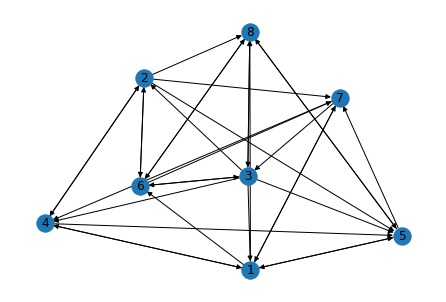
\includegraphics[scale=0.6]{img42.png}}
\caption{((3, 1), (3, 2), (3, 5), (3, 6), (4, 5)) included DiGraph}
\label{fig2}
\end{figure}

\subsection{Part (c)}
The same algorithmic search approach is also adopted to solve this part and the smallest number of edges required to achive that the node 5 becomes the first ranked node in C and node 7 becomes the first ranked node in E is 4. Result:
\[((2, 3), (3, 1), (3, 5), (4, 6))\]

It's corresponding Digraph visualization is Fig. 4.
\begin{figure}[htbp]
\centerline{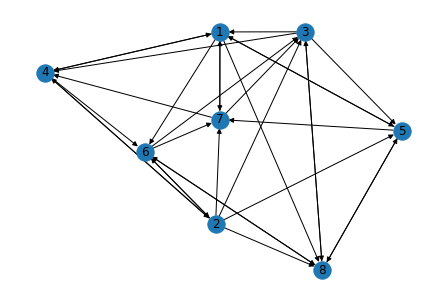
\includegraphics[scale=0.6]{img43.png}}
\caption{((2, 3), (3, 1), (3, 5), (4, 6)) included DiGraph}
\label{fig3}
\end{figure}

Note: Please refer to Question\_4.ipynb jupyter notebook for code and further details

\begin{thebibliography}{00}
\bibitem{b1} Modeling of physical network systems, Arjan van der Schaft, Johann Bernoulli Institute for Mathematics and Computer Science, Jan C. Willems Center for Systems and Control, University of Groningen.
\bibitem{b2} Optimal Sensor and Actuator Placement in
Complex Dynamical Networks, Tyler H. Summers, John Lygeros, ETH Zurich, Zurich, Switzerland.
\bibitem{b3} Grid stabilization through VSC-HVDC using wide
area measurements, Alexander Fuchs (Member, IEEE) , Sébastien Mariéthoz (Member, IEEE), Mats Larsson,
and Manfred Morari (Fellow, IEEE).
\end{thebibliography}
\vspace{12pt}
\end{document}
